% Created 2018-12-14 Fri 16:08
\documentclass[11pt]{article}
\usepackage[utf8]{inputenc}
\usepackage[T1]{fontenc}
\usepackage{fixltx2e}
\usepackage{graphicx}
\usepackage{longtable}
\usepackage{float}
\usepackage{wrapfig}
\usepackage{rotating}
\usepackage[normalem]{ulem}
\usepackage{amsmath}
\usepackage{textcomp}
\usepackage{marvosym}
\usepackage{wasysym}
\usepackage{amssymb}
\usepackage{hyperref}
\tolerance=1000
\usepackage{minted}
\usepackage[hyperref,x11names]{xcolor}
\usepackage{physics}
\usepackage{cases}
\graphicspath{ {./} }
\usepackage{tikz}
\usetikzlibrary{arrows,plotmarks,calc,positioning,fit}
\usetikzlibrary{shapes.geometric, decorations.pathmorphing, patterns, backgrounds}
\newcommand{\tikzremember}[1]{{  \tikz[remember picture,overlay]{\node (#1) at (0,11pt) { };}}}
\tikzset{snake it/.style={decorate, decoration=snake}}
\usepackage[nottoc]{tocbibind}
\author{Tigany Zarrouk}
\date{\today}
\title{things-to-do}
\hypersetup{
  pdfkeywords={},
  pdfsubject={},
  pdfcreator={Emacs 25.3.1 (Org mode 8.2.10)}}
\begin{document}

\maketitle
\tableofcontents




\section{Tasks}
\label{sec-1}

\subsection{{\bfseries\sffamily TODO} Has anyone investigated the stacking faults of Omega phase?}
\label{sec-1-1}
\begin{itemize}
\item Maybe as Omega phase doesn't occur that often, perhaps it has not been
studied in detail.
\item I should look further into this
\end{itemize}
\subsection{{\bfseries\sffamily TODO} Finish doing the gamma surfaces for all planes for pure titanium.}
\label{sec-1-2}
\subsubsection{Checking the convergence criteria}
\label{sec-1-2-1}
\begin{itemize}
\item Now checking the convergence criteria.
\end{itemize}

\begin{enumerate}
\item How the lattice parameters change with the fineness of the k mesh
\label{sec-1-2-1-1}
\begin{itemize}
\item Maybe with a less fine k mesh the lattice parameters become
worse.
\item SOLUTION: The lattice parameters do not change that much under
\end{itemize}
differences with the k mesh. \href{file:///home/tigany/Documents/disl_gsurf/hcp_pris_screw/hcp_relaxed_pris_screw/gamma_surfaces/get_hom_shear_bc_gs.py}{File with change of the lattice
parameters with k mesh. }
\href{file:///home/tigany/Documents/disl_gsurf/hcp_pris_screw/hcp_relaxed_pris_screw/gamma_surfaces/a_hcp_vs_nk.png}{a vs nk}
\href{file:///home/tigany/Documents/disl_gsurf/hcp_pris_screw/hcp_relaxed_pris_screw/gamma_surfaces/c_hcp_vs_nk.png}{c$_{\text{vs}}$$_{\text{nk}}$}
\href{file:///home/tigany/Documents/disl_gsurf/hcp_pris_screw/hcp_relaxed_pris_screw/gamma_surfaces/e_hcp_vs_nk.png}{e$_{\text{vs}}$$_{\text{nk}}$}

\begin{enumerate}
\item What if rmaxh is smaller or larger?
\label{sec-1-2-1-1-1}
\begin{itemize}
\item If rmaxh is is smaller (say rmaxh = 6.7 bohr) then we get the same
results.
\end{itemize}
\begin{figure}[htb]
\centering
\includegraphics[width=.9\linewidth]{/home/tigany/Documents/disl_gsurf/hcp_pris_screw/hcp_relaxed_pris_screw/gamma_surfaces/e_hcp_vs_nk_small_rmaxh_better_format.png}
\caption{\label{fig:e_hcp_vs_nk_small_rmaxh.png}Variation of energy with k mesh.}
\end{figure}
\begin{figure}[htb]
\centering
\includegraphics[width=.9\linewidth]{/home/tigany/Documents/disl_gsurf/hcp_pris_screw/hcp_relaxed_pris_screw/gamma_surfaces/a_hcp_vs_nk_small_rmaxh_better_format.png}
\caption{\label{fig:a-hcp_vs_nk_small_rmaxh.png}Variation of a hcp with k mesh.}
\end{figure}
\begin{figure}[htb]
\centering
\includegraphics[width=.9\linewidth]{/home/tigany/Documents/disl_gsurf/hcp_pris_screw/hcp_relaxed_pris_screw/gamma_surfaces/c_hcp_vs_nk_small_rmaxh_better_format.png}
\caption{\label{fig:c_hcp_vs_nk_small_rmaxh.png}Variation of c hcp with k mesh.}
\end{figure}]]
\begin{itemize}
\item Data: \href{file:///home/tigany/Documents/disl_gsurf/hcp_pris_screw/hcp_relaxed_pris_screw/gamma_surfaces/a_hcp_vs_nk_rmaxh_small.pkl}{a$_{\text{hcp}}$ small rmaxh}, \href{file:///home/tigany/Documents/disl_gsurf/hcp_pris_screw/hcp_relaxed_pris_screw/gamma_surfaces/c_hcp_vs_nk_rmaxh_small.pkl}{c$_{\text{hcp}}$ small rmaxh}, \href{file:///home/tigany/Documents/disl_gsurf/hcp_pris_screw/hcp_relaxed_pris_screw/gamma_surfaces/e_hcp_vs_nk_rmaxh_small.pkl}{e$_{\text{hcp}}$ small rmaxh}.
\item If rmaxh is larger ( rmaxh = 20 bohr ), all possible interactions must
be included then. And so we get the same results.
\end{itemize}
\begin{figure}[htb]
\centering
\includegraphics[width=.9\linewidth]{/home/tigany/Documents/disl_gsurf/hcp_pris_screw/hcp_relaxed_pris_screw/gamma_surfaces/e_hcp_vs_nk_large_rmaxh.png}
\caption{\label{fig:e_hcp_vs_nk_large_rmaxh.png}Variation of energy with k mesh.}
\end{figure}
\begin{figure}[htb]
\centering
\includegraphics[width=.9\linewidth]{/home/tigany/Documents/disl_gsurf/hcp_pris_screw/hcp_relaxed_pris_screw/gamma_surfaces/a_hcp_vs_nk_large_rmaxh.png}
\caption{\label{fig:a_hcp_vs_nk_large_rmaxh.png}Variation of a hcp with k mesh.}
\end{figure}
\begin{figure}[htb]
\centering
\includegraphics[width=.9\linewidth]{/home/tigany/Documents/disl_gsurf/hcp_pris_screw/hcp_relaxed_pris_screw/gamma_surfaces/c_hcp_vs_nk_large_rmaxh.png}
\caption{\label{fig:c_hcp_vs_nk_large_rmaxh.png}Variation of c hcp with k mesh.}
\end{figure}
\begin{itemize}
\item Data: \href{file:///home/tigany/Documents/disl_gsurf/hcp_pris_screw/hcp_relaxed_pris_screw/gamma_surfaces/a_hcp_vs_nk_rmaxh_large.pkl}{a$_{\text{hcp}}$ large rmaxh}, \href{file:///home/tigany/Documents/disl_gsurf/hcp_pris_screw/hcp_relaxed_pris_screw/gamma_surfaces/c_hcp_vs_nk_rmaxh_large.pkl}{c$_{\text{hcp}}$ large rmaxh}, \href{file:///home/tigany/Documents/disl_gsurf/hcp_pris_screw/hcp_relaxed_pris_screw/gamma_surfaces/e_hcp_vs_nk_rmaxh_large.pkl}{e$_{\text{hcp}}$ large rmaxh}
\end{itemize}
\end{enumerate}

\item How does rmaxh change the lattice parameters?
\label{sec-1-2-1-2}

\begin{enumerate}
\item How does rmaxh change the energy of a supercell
\label{sec-1-2-1-2-1}
\begin{itemize}
\item How does the number of neighbours change and what is the relation
between rmaxh and larger cell sizes.
\end{itemize}
\end{enumerate}
\end{enumerate}
\subsubsection{Notes on the model.}
\label{sec-1-2-2}
It seems that there is a lot of charge moving around when doing the
relaxations. 
I think that this may be due to the fact that there is no Hubbard U
interactions, a parameter for the coulomb interaction, which stops the
charges from moving freely. 
\begin{itemize}
\item TBE control file is currently set to this:
\begin{minted}[]{bash}
TBE: nbas = 128 nspec = 1 verb 31 
TB: rmaxh = 20, m-stat: F-P rlx-vol, rho 
bz: metal
\end{minted}
\end{itemize}



\subsubsection{{\bfseries\sffamily DONE} Implement Homogenous Shear boundary conditions for gamma surface calculation.}
\label{sec-1-2-3}
\subsection{{\bfseries\sffamily TODO} Python script: remove include statements  -->  One file.}
\label{sec-1-3}
\subsection{{\bfseries\sffamily TODO} Summarise UCL DFT lectures.}
\label{sec-1-4}
\subsection{{\bfseries\sffamily TODO} Write first paragraph of Literature review}
\label{sec-1-5}
\subsubsection{{\bfseries\sffamily TODO} Summarise Stacking Faults and write review}
\label{sec-1-5-1}
\subsubsection{{\bfseries\sffamily TODO} Write up the tight binding fitting of oxygen and an explanation for paramagnetism.}
\label{sec-1-5-2}
\subsubsection{{\bfseries\sffamily TODO} Summarise dislocations and Oxygen interactions (review)}
\label{sec-1-5-3}
\subsection{{\bfseries\sffamily TODO} Write summary of org-mode}
\label{sec-1-6}

\subsection{{\bfseries\sffamily DONE} Investigate why rmaxh changes energy}
\label{sec-1-7}
\begin{itemize}
\item Variation of rmaxh does not change the energy
\item Obviously the number of neighbours changes with rmaxh.
\item Conclusion: rmaxh only determines what atoms are its neighbours.
\item This is the file which investigates this:
\href{file:///home/tigany/Documents/ti/complete_titanium/ti_01-11-18/mod_rmaxh/check_rmaxh_energy_neighbours.py}{check$_{\text{rmaxh}}$$_{\text{energy}}$$_{\text{number}}$$_{\text{neighbours}}$}
\item Here is the data:
\href{file:///home/tigany/Documents/ti/complete_titanium/ti_01-11-18/mod_rmaxh/energy_for_energy_vs_rmaxh.pkl}{Energy data for energy vs rmaxh}
\href{file:///home/tigany/Documents/ti/complete_titanium/ti_01-11-18/mod_rmaxh/rmaxh_for_energy_or_n_neighbours_vs_rmaxh.pkl}{rmaxh data for energy/n$_{\text{neighbours}}$ vs rmaxh}
\href{file:///home/tigany/Documents/ti/complete_titanium/ti_01-11-18/mod_rmaxh/n_neighbours_for_n_neighbours_vs_rmaxh.pkl}{n$_{\text{neighbours}}$ for n$_{\text{neighbours}}$ vs rmaxh}
\item The output pictures are this:
\end{itemize}
\begin{figure}[htb]
\centering
\includegraphics[width=.9\linewidth]{/home/tigany/Documents/ti/complete_titanium/ti_01-11-18/mod_rmaxh/Energy_vs_rmaxh.png}
\caption{\label{fig:Energy_vs_rmaxh.png}Variation of energy with change in rmaxh}
\end{figure}
\begin{figure}[htb]
\centering
\includegraphics[width=.9\linewidth]{/home/tigany/Documents/ti/complete_titanium/ti_01-11-18/mod_rmaxh/n_neighbours_vs_rmaxh.png}
\caption{\label{fig:n_neighbours_vs_rmaxh.png}Variation of number of neighbours with change in rmaxh}
\end{figure}

\subsection{{\bfseries\sffamily DONE} Show supercell of BOP working}
\label{sec-1-8}
\subsection{{\bfseries\sffamily DONE} Check Stability Criteria}
\label{sec-1-9}
\begin{itemize}
\item Check if the matrix is complex
\item Check if it is positive definite.
\end{itemize}
\subsubsection{Results}
\label{sec-1-9-1}
\begin{itemize}
\item Without changing anything, the total energy of hcp in Tony's newest
model is $E_{\text{tot hcp}} = -0.57230068 \text{Ryd}$
\item I thought perhaps that the lattice parameters and the elastic constants
that way might produce a different result.
\item Minimising the lattice parameters gives an energy of  $E_{\text{tot
      hcp}} = -0.572351 \text{Ryd}$ with lattice parameters of
$a_{\text{hcp}} = 5.4908 \text{bohr}$, $c_{\text{hcp}} = 8.8353 \text{bohr}$ giving $c/a_{\text{hcp}} = 1.6091 \text{bohr}$
\item Elastic constants, in GPa are \[ C_{11}=185.4, C_{33}=191.8, C_{44}= 39.7, C_{12}= 56.5, C_{13}= 56.1\]
\item The stability criteria are still satisfied.
\end{itemize}
\begin{minted}[]{bash}
Checking Stability for tbe elastic constants. 
 is C_ij matrix positive definite?: True

Criteria for stability:

C_11 - C_12 > 0 
  True

C_11 + C_12 + C_33 > 0 
  True

( C_11 + C_12 ) * C_33 - 2 * C_13**2 > 0 
  True

C_44 > 0 
  True

(C_11 - C_12) > 0
  True

( C_11 + C_12 )*C_33 > 0 
  True

C_11 + C_12 > 0
  True

C_33 > 0
  True

C_11 > 0
  True
\end{minted}
\subsection{{\bfseries\sffamily DONE} Build force constant matrix for hcp}
\label{sec-1-10}
\begin{itemize}
\item If the force constant matrix is positive definite then there shan't be
any soft modes.
\end{itemize}
\subsubsection{Results}
\label{sec-1-10-1}
\begin{itemize}
\item File used is \href{file:///home/tigany/Documents/ti/complete_titanium/ti_01-11-18/check_ec_pos_definite/check_ec_pos_definite.py}{check$_{\text{ec}}$$_{\text{pos}}$$_{\text{definite}}$.py}
\item Using Fourth order $\mathcal{O}(h^{4})$ formula for the mixed
derivatives, one can find the $6\times6$ force constant matrix.
\begin{align}
  \frac{1}{144 h^2} (     &  8.  (  f_{ 1,-2} +  f_{ 2,-1} + f_{-2, 1} + f_{-1, 2} )\\
                         &-  8.  (  f_{-1,-2} +  f_{-2,-1} + f_{ 1, 2} + f_{ 2, 1} )\\
                         &-  1.  (  f_{ 2,-2} +  f_{-2, 2} - f_{-2,-2} - f_{ 2, 2} )\\
                         &+  64. (  f_{-1,-1} +  f_{ 1, 1} - f_{ 1,-1} - f_{-1, 1} )  )
\end{align}

\begin{minted}[]{bash}
Eigenvalues
[-0.3173  0.3173  2.5963 -0.3185  0.3185 -2.5963]

 Is force constant matrix positive definite? False
Force Constant Matrix
[[ 7.7099e-13  2.3901e-11 -2.3901e-11 -3.1729e-01  2.3901e-11 -2.3901e-11]
 [-7.7099e-13  0.0000e+00  0.0000e+00 -7.7099e-13 -3.1847e-01  0.0000e+00]
 [ 7.7099e-13  0.0000e+00  0.0000e+00  7.7099e-13  0.0000e+00  2.5963e+00]
 [-3.1729e-01 -2.5443e-11  2.5443e-11  2.5443e-11 -2.5443e-11  2.5443e-11]
 [-7.7099e-13 -3.1847e-01  0.0000e+00 -7.7099e-13  0.0000e+00  0.0000e+00]
 [ 7.7099e-13  0.0000e+00  2.5963e+00  7.7099e-13  0.0000e+00  0.0000e+00]]
\end{minted}

\item This matrix is not positive definite and so the structure is not
stable.

\item Using second order formula one obtains
\begin{minted}[]{bash}
Eigenvalues
[ 0.32  -0.32   2.545 -2.545  0.32  -0.32 ]

 Is force constant matrix positive definite? False
Force Constant Matrix
[[ 0.     0.     0.    -0.32   0.     0.   ]
 [ 0.     0.     0.     0.    -0.32   0.   ]
 [ 0.     0.     0.     0.     0.     2.545]
 [-0.32   0.     0.     0.     0.     0.   ]
 [ 0.    -0.32   0.     0.     0.     0.   ]
 [ 0.     0.     2.545  0.     0.     0.   ]]
\end{minted}

\item Using another model we get another matrix that is not positive
definite. 
\begin{minted}[]{bash}
tbe ti -vhcp=1  -vfddtt=0.4668418806546737 -vqddstt=0.6660968695540497 -vb0tt=94.4011791926749 
-vp0tt=1.1902574670213237 -vb1tt=-26.704816810939302 -vp1tt=0.9999600888309667 
-vcr1=-6.158653986495596 -vcr2=3.9496749559495172 -vcr3=-1.0282840982939534 
-vndt=1.992406298332605 -vahcp=5.5274  -vqq=1.5997394796830335 -vrmaxh=8.51 -vnk=30 
Eigenvalues
[ 1.8512 -1.8512  0.2823 -0.2823 -0.281   0.281 ]

 Is force constant matrix positive definite? False
Force Constant Matrix
[[-2.4672e-13 -4.8572e-13 -5.0114e-13 -2.8232e-01  0.0000e+00  1.0618e-03]
 [-4.8572e-13  0.0000e+00  0.0000e+00  0.0000e+00 -2.8103e-01  0.0000e+00]
 [-5.0114e-13  0.0000e+00  0.0000e+00  1.0618e-03  0.0000e+00  1.8512e+00]
 [-2.8232e-01  0.0000e+00  1.0618e-03 -2.5443e-13  0.0000e+00 -1.0618e-03]
 [ 0.0000e+00 -2.8103e-01  2.4672e-13  0.0000e+00  0.0000e+00  0.0000e+00]
 [ 1.0618e-03 -2.4672e-13  1.8512e+00 -1.0618e-03 -2.4672e-13 -7.4015e-13]]
\end{minted}
\end{itemize}

\subsection{{\bfseries\sffamily TODO} Make dislocations go through centre of triangle of atoms}
\label{sec-1-11}

\subsection{{\bfseries\sffamily TODO} Investigate why the gamma surface minima are not along the lines joining the vectors.}
\label{sec-1-12}

\subsection{{\bfseries\sffamily TODO} Change the lattice vectors to make the dislocation displacement fields periodic}
\label{sec-1-13}

\subsection{{\bfseries\sffamily TODO} Make sure that the displacements are periodic}
\label{sec-1-14}

\subsection{{\bfseries\sffamily TODO} Why is the displacement in the x direction in the graphs of create cells?}
\label{sec-1-15}
\subsection{{\bfseries\sffamily TODO} Calculate the Internal elastic constants, like in Cousins \cite{Cousins1979}}
\label{sec-1-16}
\section{General notes}
\label{sec-2}
\subsection{Dislocation arrays}
\label{sec-2-1}
Dislocation arrays are used within simulation cells to negate the effects of
the long range strain fields produced from dislocations in the periodic array
of cells one has in the simulation.
\begin{itemize}
\item Method of Clouet: Dislocation locking versus easy glide in titanium and
zirconium. \cite{Clouet2015} 
\begin{itemize}
\item Introduced two dislocations into the simulation cell
\item This formed a quadrupolar periodic array of dislocations which
minimises the elastic interaction between dislocations and their
images.
\item This is because of the centrosymmetry of the Volterra elastic field,
which means that the stress of this quadrupolar array ensures that the
stress field created by the periodic image dislocations cancels locally
at each dislocation position, thus limiting the perturbation of the
dislocation core by the boundary conditions.
\item Arrangement is the same as the "S" arrangement found in
\cite{Clouet2012}
\end{itemize}
\end{itemize}

\subsubsection{Files to produce dislocations}
\label{sec-2-1-1}
\begin{enumerate}
\item Single Dislocations
\label{sec-2-1-1-1}
Here are the files used to produce single dislocations
\href{file:///home/tigany/Documents/disl_gsurf/useful_python/bop/dislocations/create_dislocations/gen_prismatic_screw_tbe.py}{Generate prismatic screw} \href{file:///home/tigany/Documents/disl_gsurf/useful_python/bop/dislocations/create_dislocations/test/generated_dislocations/site.ti_9x_9y_8z_square_1_dislanis_prim_rot_convert.xyz}{Ovito file }
\href{file:///home/tigany/Pictures/prismatic_screw_tbe_full_anis.png}{prismatic screw from ovito }
\item Quadrupolar arrangements
\label{sec-2-1-1-2}
\end{enumerate}

\subsubsection{Bulatov and Cai: Computer simulations of dislocations}
\label{sec-2-1-2}

\begin{enumerate}
\item Sum of displacements from dipoles
\label{sec-2-1-2-1}
Simulating dislocation dipoles will introduce singularity in displacement
between them. As we are not in the continuous case, this singularity is
fine. However, the periodic boundary conditions are \textbf{not} satisfied,
\emph{i.e.} pair of dislocations forming a dipole will not be periodic
along y, as the displacement field is not periodic along y. 

This mismatch could relax away during energy minimization, but it is not
guaranteed. 

A naive way to try and remove this result is to try and construct a
periodic displacement field from the non-periodic one generated, by the
principle of linear superposition, but this does not work. 
\[ u_{z}^{\text{sum}} = \sum_{\mathbf{R}} u_{z}^{\inf}(\mathbf{r}
     -\mathbf{R}) = u_{z}^{\inf}(\mathbf{r}) + u_{z}^{\text{img}}(\mathbf{r})
     \]
\[  u_{z}^{\text{img}}(\mathbf{r}) = \sum_{\mathbf{R}}' u_{z}^{\inf}(\mathbf{r}
     -\mathbf{R}) \]

where $\mathbf{R}$ is a periodic vector of the two dimensional lattice
vectors along $x$ and $y$ axes: $\mathbf{R} = n_{1}\mathbf{c}_1 +
     n_{2}\mathbf{c}_2$.
$u_{z}^{\text{img}}(\mathbf{r})$ only accounts for \textbf{image} dipoles
($\mathbf{R}\neq 0$)
whereas the other sum is the sum of all of them. 
This is because the sum of the displacements is \emph{conditionally
convergent}. This means that the ordering of the sum of the displacements
will determine if the sum actually converges.

\item How to remove non-periodic displacements
\label{sec-2-1-2-2}
One can find the periodic displacement $u_{z}^{text{PBC}}(\mathbf{r})$
from the relation, which arises from the fact that
$\partial_{i}\partial_{j}u_{z}^{\text{sum}}(\mathbf{r}) = \partial_{i}\partial_{j}u_{z}^{\text{PBC}}(\mathbf{r})$
\[ u_{z}^{text{sum}}(\mathbf{r}) =  u_{z}^{text{PBC}}(\mathbf{r}) +
     \mathbf{s}\cdot\mathbf{r} + \mathbf{u}_{0} \]
$\mathbf{u}_{0}$ is a constant term, so it can be ignored. 

Recipe to remove the spurious non-periodic part of the displacement field:
\begin{enumerate}
\item Evaluate the conditionally convergent sum
$u_{z}^{\text{sum}}(\mathbf{r})$, using an arbitrary truncation.
\item "Measure" the linear spurious part of the resulting field, using the
equation below, by comparing it's values at four points in the
periodic supercell from the above equation 
\[ u_{z}^{\text{err}}(\mathbf{r}) =  \mathbf{s}\cdot\mathbf{r},  \]
\[ u_{z}^{\text{sum}}(\mathbf{r} + \mathbf{c}_{i})  -
        u_{z}^{\text{sum}}(\mathbf{r}) = \mathbf{s}\cdot\mathbf{c}_{i}, \]
where $i=1,2$.
\item Finally, subtract the linear term $u_{z}^{\text{err}}(\mathbf{r})$ from
$u_{z}^{\text{sum}}(\mathbf{r})$ to obtain the corrected solution
$u_{z}^{\text{PBC}}(\mathbf{r})$.
\end{enumerate}


This procedure is independent of the truncation in the limit of large
radius.

\item Adjusting the shape of the supercell
\label{sec-2-1-2-3}
When a dislocation dipole is introduced, there is a plastic strain that
is generated. 
\[ \epsilon^{\text{pl}} = \frac{1}{2\Omega}( \mathbf{b} \otimes
     \mathbf{A} + \mathbf{A} \otimes \mathbf{b} ), \]
where $\Omega = (\mathbf{c}_{1} \times \mathbf{c}_{2}) \cdot
     \mathbf{c}_{3}$, and $\mathbf{A}$, is the vector normal to the plane of
the plane connecting the dipoles and $\mathbf{c}_{i}$ are the periodicity vectors. 

In a supercell with fixed periodicity vectors, an increment in the
plastic strain will be compensated by an oppositely signed increment of
the elastic strain of the same magnitude: $\epsilon^{\text{el}} = -
     \epsilon^{\text{pl}}$.

In response to this elastic strain, there will be an internal
\emph{back-stress} acting to eliminate the source of the strain (i.e. the
dislocation dipole). This back-stress may be large enought to push the
dislocations back from their intended positions and may even lead to
dislocation recombination. 

Allowing for the simulation box to change shape during relaxation, one
would see that it could reach a state of zero average internal stress. 
We can do this step \textbf{before relaxation}, such that we can accomodate/match the
\textbf{plastic strain} produced by the dislocation dipole.

In the case study, the cut plane bounded by two dislocations is parallel
to two of the repeat vectors, $\mathbf{c}_{1}$ and $\mathbf{c}_{3}$. In
this case the internal stress induced by the dipole can be removed by
adjusting only the $\mathbf{c}_{2}$ repeat vector. 

\[ \mathbf{c}_{2} \rightarrow \mathbf{c}_{2} + \mathbf{b} \frac{A}{A_{0},} \]

If we say that $A_{0} = | \mathbf{c}_{3} \times \mathbf{c}_{1} |$ is the area of simulation box on the plane
parallel to the dislocation dipoles, and $A$ is the area that is between
the dislocation dipoles in the simulation cell. 

Adjusting this vector means that we have added an extra term
$\mathbf{u}_{z}^{\text{tilt}}(\mathbf{r})$ to the solution of
$\mathbf{u}_{z}^{\text{PBC}}(\mathbf{r})$ from before. 
In this study, it is 
\[ u_{z}^{\text{tilt}}(\mathbf{r}) = b \frac{Ay}{A_{0}c_{2}}, \]
where $c_{2}$ is the length of the periodicity vector before it has been
tilted.
\end{enumerate}


\subsection{TBE Pair potentials and Bond integrals}
\label{sec-2-2}
\subsubsection{Pair potentials in tbe code}
\label{sec-2-2-1}
\begin{itemize}
\item Pair potential is constructed by \href{file:///home/tigany/lm/tb/makvpp.f}{makvpp.f}.
\item This calls \href{file:///home/tigany/lm/tb/vppder.f}{vppder.f} which actually evaluates the pair potential at that
point
\item In makvpp.f, if in the range of $r_1 < r < r_{\text{c}}$, then
augmentative/multiplicative polynomial is used.
\begin{itemize}
\item To make this polynomial \href{file:///home/tigany/lm/tb/pcut45.f}{pcut45.f} is used.
\item Depending on the degree of polynomial we have this structure:
\begin{minted}[]{fortran}
      rr = r1 - r2
      xr1 = x - r1
      xr2 = x - r2

      c = val*rr*rr
      if (n == 5) then
	pnorm = rr**(-5)
	a = (0.5d0*curv*rr - 3d0*slo)*rr + 6d0*val
	b = (slo*rr - 3d0*val)*rr
      elseif (n == 4) then
	pnorm = rr**(-4)
	a = (0.5d0*curv*rr - 2d0*slo)*rr + 3d0*val
	b = (slo*rr - 2d0*val)*rr
      p2 = pnorm*(c + xr1*(b + xr1*a))
      dp2 = pnorm*(b + xr1*2d0*a)
      ddp2 = pnorm*2d0*a
      e = p2 * xr2**(n-2)
      de = (xr2*dp2 + float(n-2)*p2) * xr2**(n-3)
      dde = (xr2*xr2*ddp2+float(2*(n-2))*xr2*dp2+float((n-2)*(n-3))*p2)
C ... e, de and dde are the values and derivatives of the polynomial in the region r1 , r < rc
\end{minted}
\item So the form of the polynomial used is
\begin{itemize}
\item $$ P_5(x) = (x-r_2)^3 P_2(x)  $$
\item \[ P_2(x) = a(x-r1)^2 + b(x-r_1) + c \]
\item \[ a = \frac{1}{ (r1-r2)^5 } \big\{  \frac{1}{2}(r_1-r_2)^2f"(r_1) -3(r_1-r_2)f'(r_1) + 6f(r_1) \big\} \]
\item \[  b = \frac{1}{(r_1-r_2)^4} \big\{ f'(r_1)*(r_1-r_2) - 3f(r_1) \big\}  \]
\item \[ \frac{1}{(r_1 - r_2)^5} x \]
\item \[  c = \frac{ f(r_1) }{ (r_1-r_2)^3} \]
\item Where $f(x)$ is the function that needs to be cut
\end{itemize}
\end{itemize}
\item Current model has this
\begin{minted}[]{bash}
Ti,Ti:
   type 2 (Exp. decay), V(d) = a exp (- b d)
	     dds    ddp    ddd
   coeff:  -2.75   1.84  -0.46
   decay:   0.71   0.71   0.71
   cutoff type 2 (multiplicative), 5th order polynomial, range [r1, rc]
	     dds    ddp    ddd
   r1:      6.20   6.20   6.20
   rc:      8.50   8.50   8.50
\end{minted}
\end{itemize}



\subsubsection{Bond integrals from tbe}
\label{sec-2-2-2}
\begin{itemize}
\item So bond integrals from titanium look like this, from this file
\href{file:///home/tigany/Documents/ti/complete_titanium/ti_01-11-18/plot_bond_integrals/plot_bond_integrals.py}{plot$_{\text{bond}}$$_{\text{integrals}}$.py}
\end{itemize}
\begin{figure}[htb]
\centering
\includegraphics[width=.9\linewidth]{/home/tigany/Documents/ti/complete_titanium/ti_01-11-18/plot_bond_integrals/tbe_bond_integrals_with_polynomial_cutoffs_multiplicative_alt.png}
\caption{\label{fig:tbe_bond_integrals_with_polynomial_cutoffs_multiplicative_alt.png}Bond integrals with multiplicative polynomial cutoffs.}
\end{figure}
\begin{figure}[htb]
\centering
\includegraphics[width=.9\linewidth]{/home/tigany/Documents/ti/complete_titanium/ti_01-11-18/plot_bond_integrals/tbe_bond_integrals_with_polynomial_cutoffs_multiplicative_zoomed_in.png}
\caption{\label{fig:tbe_bond_integrals_with_polynomial_cutoffs_multiplicative_zoomed_in.png}Bond integrals with multiplicative polynomial cutoffs: zoomed in.}
\end{figure}

\subsubsection{Bond Integrals for first neighbour interaction}
\label{sec-2-2-3}
To make first neighbours it is optimal to have a cutoff that is within
alat and \$1.4 \texttimes{} \$ alat. This is within the next shell of 6 neighbours
and so having the cutoff between alat and $1.2\times$ alat should be
optimal. 
\begin{figure}[htb]
\centering
\includegraphics[width=.9\linewidth]{/home/tigany/Documents/ti/complete_titanium/ti_01-11-18/plot_bond_integrals/check_new_cutoffs/cutoffs_at_alat_and_one_point_four_alat.png}
\caption{\label{fig:tbe_bond_integrals_new__with_polynomial_cutoffs_multiplicative_zoomed_in.png}Bond integrals with multiplicative polynomial cutoffs for first neighbour interactions: zoomed in.}
\end{figure}

\subsection{Force constant matrix}
\label{sec-2-3}
\subsubsection{Wallace}
\label{sec-2-3-1}
\begin{enumerate}
\item Crystal Potential: Introduction
\label{sec-2-3-1-1}
\begin{itemize}
\item Since the vibrational energy of a crystal is generally considered to by
small compared to its potential energy, the crystal potential is a first
approximation to the free energy or the internal energy.
\item Ions are labelled by the letters $M$ and $N$.
\item Equilibrium positions are given by the vectors $\mathbf{R}(M)$ and
displacements from equilibrium are denoted by $\mathbf{U}(M)$.
\item Potential energy of the crystal due to interactions among ions in a
given configuration is given by $\Phi$, which can be expanded as
\begin{align}
\Phi = \Phi_{0} &+ \sum_{M}\sum_{i} \Phi_{i}(M)U_{i}(M) \\ 
     &+ \frac{1}{2}\sum_{MN}\sum_{ij}\Phi_{ij}(M,N)U_i(M)U_j(N)\\ 
     &+ \frac{1}{3!} \sum_{MNP}\sum_{ijk}\Phi_{ijk}(M,N,P)U_{i}(M)U_{j}(N)U_{k}(P) \\
     &+ \frac{1}{4!} \sum_{MNPQ}\sum_{ijkl}\Phi_{ijkl}(M,N,P,Q)U_{i}(M)U_{j}(N)U_{k}(P)U_{l}(Q) + \dots \\
\end{align}
\item $\Phi_{i}(M) = \frac{\partial \Phi}{\partial U_{i}(M)}$
\item $\Phi_{ij}(M) = \frac{\partial^{2} \Phi}{\partial U_{i}(M)U_{j}(N)}$
\item These are symmetric in their index pairs; \emph{i.e.} $\Phi_{ij}(M,N) = \Phi_{ji}(N,M)$
\item All of the coefficients are functions of the \emph{initial} configuration.
\item This potential is supposed to represent the \emph{entire} energy of the crystal
except for the kinetic energy of the ions.
\item From now on $M, N$ represent the unit cell and $\mu, \nu$ represent the
individual ions in a given cell.
\item The total potential of the system plus externally applied forces is
$\Psi$. For a virtual process where the crystal is deformed while the
externally applies forces are held constant $\Psi$ is not conserved, if
the forces are changed then it can be conserved. 
\begin{align}
\Psi = \Psi_{0} &+ \sum_{M}\sum_{i}[\Phi_{i}(M) - f_i(M)]U_{i}(M)\\
     &+ \frac{1}{2}\sum_{MN}\sum_{ij}\Phi_{ij}(M,N)U_i(M)U_j(N) \dots
\end{align}
\end{itemize}
\item Stability and the Dynamical Matrix
\label{sec-2-3-1-2}
\begin{itemize}
\item The equilibrium configuration of ions and external forces is a stable
equilibrium if the total system potential is minimum with respet to
small virtual displacements of the ions from equilirium.
\end{itemize}
\[\Psi = \Psi_{0}+
     \frac{1}{2}\sum_{MN}\sum_{ij}\Phi_{ij}(M,N)U_i(M)U_j(N) + \dots \]
\begin{itemize}
\item The stability condition is if they are positive definite: positive for
any of the values $U_{i}(M)$, except if they are all 0.
\item The stability condition is:
\[ \sum_{\alpha \beta} \Phi_{\alpha\beta}U_{\alpha}U_{\beta} > 0 \]
\item $\alpha$, $\beta \dots$ are indices which refer to the pair  $Mi$ and
$>0$ means positive definite (all the eigenvalues are greater than zero).
\item This is only satisfied if the matrix $\Phi_{\alpha\beta}$ is positive definite.
\end{itemize}
\end{enumerate}
\subsection{Gamma surfaces}
\label{sec-2-4}
\subsubsection{Miscellaneous}
\label{sec-2-4-1}
\begin{itemize}
\item Seems like some atoms are missing in the site file when it is being read
in to tbe.
\item This means that there are some erroneous forces that make the program
exit.
\begin{itemize}
\item SOLUTION: Coordinates were not in units of alat.
\end{itemize}
\end{itemize}
\subsubsection{Relaxing in tbe}
\label{sec-2-4-2}
\begin{itemize}
\item To relax in tbe need to modify:
\begin{itemize}
\item Ewald tolerance: ewtol
\begin{itemize}
\item This can generally be set quite low: 1d-14
\end{itemize}
\item Convergence criteria:
\begin{itemize}
\item gtol: The tolerance in the force for convergence e.g. 1d-8
\item xtol: The tolerance in the atomic positon e.g. 1d-8.
\end{itemize}
\end{itemize}
\end{itemize}

\subsubsection{Convergence and k-points in tbe}
\label{sec-2-4-3}
\begin{itemize}
\item Tony used a $30\times 30\times 30$ grid for the k-point mesh.
\item Making a square cell, and increasing the length accordingly, one must
reduce the number ok k-points in that direction.
\item Making a square cell with an increase of cell size along x to be
$\sqrt{3}$, then we must reduce the k-point mesh by $n_{\text{kx}} /
      \sqrt{3} \approx 17.3 \approx 17$
\item Therefore new grid is $17 \times 30 \times 30$
\end{itemize}

\begin{center}
\begin{tabular}{lrrrrrrrrrr}
hcp cell type & Geometry & tetra & n atoms & nkx & nky & nkz & Maximum force & Total energy per atom & Band energy per atom & Pair pot. energy per atom\\
\hline
Primitive & 1x1x1 & 0 & 2 & 30 & 30 & 30 & 0.000000 & -0.28614958 & -0.93606433 & 0.18636598\\
Primitive & 1x1x1 & 1 & 2 & 30 & 30 & 30 & 0.000001 & -0.28614745 & -0.93606220 & 0.18636599\\
Primitive & 2x1x1 & 0 & 4 & 15 & 30 & 30 & 0.000001 & -0.28614836 & -0.93606433 & 0.18636599\\
Primitive & 2x1x1 & 1 & 4 & 15 & 30 & 30 & 0.000511 & -0.28614581 & -0.93606056 & 0.18636599\\
Primitive & 4x2x8 & 0 & 128 & 8 & 15 & 4 & 0.000061 & -0.28615991 & -0.93607466 & 0.18636599\\
Primitive & 4x2x8 & 1 & 128 & 8 & 15 & 4 & 0.000118 & -0.28615978 & -0.93607452 & 0.18536599\\
Primitive & 4x2x8 & 0 & 128 & 9 & 15 & 4 & 0.000063 & -0.28614977 & -0.93606452 & 0.18636599\\
Basal Square & 1x1x1 & 0 & 4 & 16 & 30 & 30 & 0.000065 & -0.28614681 & -0.93606156 & 0.18636599\\
Basal Square & 1x1x1 & 0 & 4 & 17 & 30 & 30 & 0.000064 & -0.28615864 & -0.93607339 & 0.18636599\\
Basal Square & 1x1x1 & 0 & 4 & 18 & 30 & 30 & 0.000043 & -0.28614481 & -0.93605956 & 0.18636599\\
Basal Square & 1x1x1 & 0 & 4 & 19 & 30 & 30 & 0.000054 & -0.28615677 & -0.93607152 & 0.18636599\\
Basal Square & 1x2x8 & 0 & 64 & 15 & 15 & 30 & 0.000083 & -0.28615743 & -0.93606721 & 0.18636599\\
Basal Square & 1x2x8 & 0 & 64 & 16 & 15 & 30 & 0.000020 & -0.28614599 & -0.93606074 & 0.18636599\\
Basal Square & 1x2x8 & 0 & 64 & 17 & 15 & 30 & 0.000061 & -0.28615547 & -0.93607022 & 0.18636599\\
Basal Square & 1x2x8 & 0 & 64 & 18 & 15 & 30 & 0.000057 & -0.28614492 & -0.93605967 & 0.18636599\\
Basal Square & 1x2x8 & 0 & 64 & 15 & 15 & 4 & 0.000065 & -0.28615784 & -0.93607259 & 0.18636599\\
Basal Square & 1x2x8 & 0 & 64 & 16 & 15 & 4 & 0.000028 & -0.28614667 & -0.93606014 & 0.18636599\\
Basal Square & 1x2x8 & 0 & 64 & 17 & 15 & 4 & 0.000044 & -0.28615651 & -0.93607126 & 0.18636599\\
Basal Square & 1x2x8 & 0 & 64 & 18 & 15 & 4 & 0.000052 & -0.28614359 & -0.93605834 & 0.18636599\\
Basal Square & 1x2x10 & 0 & 80 & 15 & 15 & 3 & 0.000087 & -0.28615445 & -0.93606920 & 0.18636599\\
Basal Square & 1x2x10 & 0 & 80 & 16 & 15 & 3 & 0.000065 & -0.28614681 & -0.93606156 & 0.18636599\\
Basal Square & 1x2x10 & 0 & 80 & 17 & 15 & 3 & 0.000064 & -0.28615864 & -0.93607343 & 0.18636599\\
Basal Square & 1x2x10 & 0 & 80 & 18 & 15 & 3 & 0.000052 & -0.28614359 & -0.93605834 & 0.18636599\\
\end{tabular}
\end{center}
Less precise c/a below. 
\begin{center}
\begin{tabular}{lrrrrrrrrr}
\hline
Basal Square  1x1x1 & 0 & 4 & 18 & 30 & 30 & 0.000043 & -0.28614662 & -0.93605957 & 0.18636601\\
Basal Square  1x1x1 & 1 & 4 & 18 & 30 & 30 & 0.000097 & -0.28614928 & -0.93606369 & 0.18636601\\
Basal Square  1x1x1 & 0 & 4 & 17 & 30 & 30 & 0.000064 & -0.28615864 & -0.93607342 & 0.18636601\\
Basal Square  1x1x1 & 1 & 4 & 17 & 30 & 30 & 0.000024 & -0.28615254 & -0.93606731 & 0.18636601\\
Basal Square: 2x2x8 & 0 & 128 & 9 & 15 & 4 & 0.000052 & -0.28614359 & -0.93605835 & 0.18366000\\
Basal Square: 2x2x8 & 1 & 128 & 9 & 15 & 4 & 0.000121 & -0.28614669 & -0.93606145 & 0.18636600\\
Basal Square: 1x1x8 & 0 & 32 & 17 & 30 & 4 & 0.000044 & -0.28615651 & -0.93607127 & 0.18636600\\
Basal Square: 1x1x9 & 0 & 36 & 17 & 30 & 4 & 0.000058 & -0.28615716 & -0.93607192 & 0.18636600\\
Basal Square: 1x1x9 & 0 & 36 & 17 & 30 & 3 & 0.000071 & -0.28615681 & -0.93607157 & 0.18636600\\
\end{tabular}
\end{center}

\subsubsection{Results}
\label{sec-2-4-4}
\begin{itemize}
\item Have now done the gamma line along $1/3[1\bar{2}10]$, but the end points
do not seem quite right.
\item File and data: \href{file:///home/tigany/Documents/disl_gsurf/hcp_pris_screw/hcp_relaxed_pris_screw/gamma_surfaces/data/plot_hsbc_pkl.py}{basal$_{\text{energy}}$$_{\text{plotting}}$} \includegraphics[width=.9\linewidth]{/home/tigany/Documents/disl_gsurf/hcp_pris_screw/hcp_relaxed_pris_screw/gamma_surfaces/data/gamma_line_along_1-210_wrong_endpoints.png}
\item Basal plot $8\times 8\times 8$
\item \href{file:///home/tigany/Documents/disl_gsurf/hcp_pris_screw/hcp_relaxed_pris_screw/gamma_surfaces/data/supercell_8-8-8/Figures/gamma_surface_8-8-8_basal_tbe.png}{Basal Plane gamma surface}
\item \href{file:///home/tigany/Documents/disl_gsurf/hcp_pris_screw/hcp_relaxed_pris_screw/gamma_surfaces/data/supercell_8-8-8/plot_hsbc_pkl.py}{plot$_{\text{hbgs}}$}, \href{file:///home/tigany/Documents/disl_gsurf/hcp_pris_screw/hcp_relaxed_pris_screw/gamma_surfaces/data/supercell_8-8-8/hgsBte888.pkl}{energy}, \href{file:///home/tigany/Documents/disl_gsurf/hcp_pris_screw/hcp_relaxed_pris_screw/gamma_surfaces/data/supercell_8-8-8/hgsBtx888.pkl}{x}, \href{file:///home/tigany/Documents/disl_gsurf/hcp_pris_screw/hcp_relaxed_pris_screw/gamma_surfaces/data/supercell_8-8-8/hgsBty888.pkl}{y}
\end{itemize}


\subsubsection{Literature Review}
\label{sec-2-4-5}

\begin{enumerate}
\item General notes on dislocations
\label{sec-2-4-5-1}
\begin{itemize}
\item Dislocations have areas of tension (distance between atoms is larger
than the lattice vector) and compression (distance is less than the
lattice vector)
\item A reasonable value for the dislocation core radius r0 therefore lies in the range $\mathbf{b}$ to $4\mathbf{b}$, i.e. $r_0 \geq 1 nm$ in most cases.
\end{itemize}

\item How do stacking faults occur?
\label{sec-2-4-5-2}
Stacking faults can occur:
\begin{itemize}
\item During crystal growth
\item As part of other defects (e.g. dislocations)
\item As evolution of other defects.
\begin{itemize}
\item There can be vacancy agglomeration, such that there is a vacancy
disk, creating a stacking fault if the disk is large enough for the
two surfaces to collapse together.
\item Example of this is that these vacancy disks condense and are then
bordered by an edge dislocation.
\end{itemize}
\end{itemize}

\item Types of stacking faults.
\label{sec-2-4-5-3}
\begin{itemize}
\item Disk of vacancies: \emph{intrinsic} stacking fault.
\item Interstitial agglomeration: \emph{extrinsic} stacking fault.
\item Both are bordered by an edge dislocation.
\begin{itemize}
\item These are \emph{partial} dislocations.
\item In fcc these are Frank partials of burgers vector $\mathbf{b} =
         \pm \frac{a}{3}\langle 111\rangle$
\end{itemize}
\end{itemize}

\begin{enumerate}
\item Types of stacking faults in hcp
\label{sec-2-4-5-3-1}
\begin{itemize}
\item Intrinsic 1 ($I_1$) = (ABAB|CBCB) -- Basal plane
\item Intrinsic 2 ($I_2$) = (ABAB|CACA) -- Basal plane
\item Extrinsic ($I_{\text{E}}$) = (ABAB|C|ABAB) -- Basal plane
\item Easy prismatic $F_{1} = \mathbf{b} / 2$
\begin{itemize}
\item This energy corresponds to a true metastable stacking fault but has
only been seen in the case of DFT so far.
\end{itemize}
\end{itemize}
\end{enumerate}

\item Partial dislocations
\label{sec-2-4-5-4}
\begin{itemize}
\item Partial dislocations \emph{must} be bordered by a two dimensional
defect: usually a stacking fault.
\begin{itemize}
\item (Think of double ended pencil slice, where dislocation lines are the
border of the pencil and the plane is the stacking fault.)
\end{itemize}
\item Shockley dislocations:
\begin{itemize}
\item Cut and weld but don't fill in (to finish full Volterra procedure.)
\item Produce intrisic stacking fault.
\item These can glide on the same plane as the perfect dislocation, and can
also change length.
\item Frank partials bound loop and so can only move on their glide
cylinder. Changing length would involbe apsorption or emission of
point defects.
\end{itemize}
\end{itemize}

\item Energy considerations with stacking faults and partials.
\label{sec-2-4-5-5}
\begin{itemize}
\item Have energy gain from splitting into two smaller burgers vectors
\item Interaction energy of two partials will be large at smaller distances
\item but also, stacking fault energy is per unit length, so this would
minimise the distance
\item So have an equilibrium distance between the partials.
\item This makes dislocations like ribbons that stretch through the material.
\item These ribbons can undergo constrictions from jogs
\item Reason that stacking faults are not observed in bcc structures are just
that the stacking fault energies are too high. (Because of dense packing?)
\end{itemize}
\item Gamma surfaces in DFT
\label{sec-2-4-5-6}
\begin{enumerate}
\item\relax [Benoit, Tarrat and Morillo 2012] Density functional theory investigations of titanium $\gamma$-surfaces and stacking faults.
\label{sec-2-4-5-6-1}
\begin{itemize}
\item Comparison between central force  embedded atom ineractions, N-body
central force, N-body angular, empirical potentials, tight binding and
DFT pseudopotential and DFT full electron calculations.
\item Cauchy pressures are deemed to due to be N-body effects but really for Cauchy
pressures that are accurate one needs a volume-dependent energy term
which makes elastic constant contributions. \textbf{\textbf{Needs more investigation}}
\item Legrand suggests that there is an energetic favouring of the prismatic
plane for these stacking fault energies due to the directional covalent
d-orbital bonding in transition metals.
\item He also suggested a ratio to measure this \[ R = \frac{\gamma_{b}/C_{44}}{\gamma_{p}/C_{66}} \].
\item Suggests that large fitting database of configurations far from the
ideal hcp lattice might provide accurate reproduction of dislocation
core structure.
\item Not systematic improvement going from N-body central force potentials
to TB.
\item Inversion in strength between $C_{66}$ and $C_{44}$ in the BOP
calculations of Girshick and Pettifor
\begin{itemize}
\item So it was stipulated that the N-body effects of this model were not
well accounted for.
\end{itemize}
\item Free surfaces were introduced into the slab geometry to avoid problems
of asymmetric configuration of stacking faults in periodic images.
\item Oscillations in the stacking fault energy with the number of slabs are
due to quantum size effects.
\item Underestimation of the energy of basal faults and overestimation of the
prismatic easy excess energy lead to an inversion between the basal and
prismatic easy faults in terms of energetic preference. This was also
seen in the BOP model.  
\begin{itemize}
\item Not sure how this works. The Cauchy pressure was fitted to in certain
BOP models. Maybe this was only used in Stefan Znam's case and not
any others. It would be interesting to see if his model stands up
against this criteria.
\end{itemize}
\item No models other than DFT produced a metastable stacking fault energy at
the prismatic easy fault.
\end{itemize}
\end{enumerate}
\end{enumerate}
\subsection{Notes on Thermodynamics and Stability}
\label{sec-2-5}

\subsubsection{Wallace 1972}
\label{sec-2-5-1}
\begin{itemize}
\item For hexagonal materials, there are general stability requirements:
\begin{itemize}
\item $C_{11} - C_{12} > 0$
\item $C_{11} + C_{12} + C_{33} > 0$
\item $( C_{11} + C_{12} ) C_{33} - 2C_{13}^{2} > 0$
\item $C_{44} > 0$
\item $C_{66} = \frac{1}{2}(C_{11} - C_{12}) > 0$
\item $( C_{11} + C_{12} )C_{33} > 0$
\item $C_{11} + C_{12} > 0$
\item $C_{33} > 0$
\item $C_{11} > 0$
\end{itemize}
\item The equilibrium configuration of ions plus external forces is a stable
equilibrium if the total system potential $\Psi$ is minimum with respect
to small virtual displacements of dions from equilibrium.
\item Cauchy relations (at least in the cubic case) will be destroyed if
non-central forces are included in the crystal potential.
\end{itemize}

\subsubsection{Fast, Will, Johansson: Elastic constants in hexagonal transition metals}
\label{sec-2-5-2}

\begin{enumerate}
\item Cauchy Relations
\label{sec-2-5-2-1}
\begin{itemize}
\item Cauchy relations for hexagonal materials:
\begin{itemize}
\item $C_{13} = C_{44}$
\item $C_{12} = C_{66} = \frac{1}{2}(C_{11} - C_{12})$
\end{itemize}
\item These only are meant to hold for central forces.
\item These Cauchy forces have been shown to hold more in hexagonal materials
rather than cubic ones.
\item In cubic materials sometimes one finds $C_{44}$ four times smaller than
$C_{12}$.
\item They showed the Cauchy ratios:
\begin{itemize}
\item $C_{12}/C_{66}$
\item $C_{13}/C_{44}$
\end{itemize}
\item The Cauchy relations were close to 1 apart from calculations with Co, Zr and
Ti, where it was closer to 2.
\item These are smaller than the $3/4$ times deviations in cubic crystals.
\end{itemize}

\item Normalised elastic constant
\label{sec-2-5-2-2}
\begin{itemize}
\item To investigate Cauchy relations fully they used a normalised elastic constant which
was obtained by dividiing by the bulk modulus: $C'_{ij} = C_{ij}/B$
\item It becomes easier to study trends as one is normlising the
interatomic forces with an average restoring force of the system,
when dividing by the bulk modulus.
\item Suggest that the hexagonal materials are quite isotropic.
\end{itemize}
\end{enumerate}
\subsection{Notes on Tight Binding and BOP Models}
\label{sec-2-6}

\subsubsection{Pair correlation and cutoffs}
\label{sec-2-6-1}
\begin{itemize}
\item Analysing the pair correlation function in ovito, it seems reasonable
that one should have cutoffs, if \$ a = 2.95 \$ and \$ c = 4.683\$ to give a
$c/a = 1.587$, of 4.7$\AA$, as this is past the third neighbour
distance.
\item This was done in Znam's thesis.
\item At the moment we are cutting off at $8.5 ryd$, which gives the
neighbours to be 20, so we are actually not including a multiple of the
coordination for the neighbour table, which may give a weird structure
by symmetry.
\item Another reason is that in the model for Titania, the Ti-Ti integrals
were given a longer cutoff to stabilise the rutile and anatase
structures.
\item The TB Iron model has a cutoff which is twice the lattice parameter.
\end{itemize}
\subsubsection{Trinkle 2006}
\label{sec-2-6-2}
\begin{itemize}
\item Collapse problem found in tight binding if atoms come too close
together. Electrons go in the bonding state and not the anti-bonding
state and so the energy goes down
\item Can be fixed by implementing spline potential that levels off below a
given cutoff, which effectively simulates a pair potential.
\item Environmentally dependent on-site terms were used instead of a pair potential.
\item These on-site energies are dependent on the local density $\rho_{i}$ and
they have a cutoff function $f_{c}(r_{ij})$ which has fixed parameters
$R_{0}$ and $l_{0}$.\[
      \epsilon_{i,l} = a_{l} + b_{l}\rho_{i}^{2/3} + c_{l}\rho_{i}^{4/3} +
      d_{l}\rho_{i}^{2}\] 
\[ \rho_{i} = \sum_{j \neq i} \text{exp}\big\{ -\lambda^{2} r_{ij}
      f_{c}(r_{ij}) \big\} \]
\[ f_{c}(r) = \frac{1}{1 + \text{exp}\Big\{  \frac{r-R_{0}}{l_{0}}\Big\}
      }\]
\end{itemize}
\subsubsection{Stefan Znam 2001 Thesis}
\label{sec-2-6-3}
\begin{enumerate}
\item Cauchy Pressures
\label{sec-2-6-3-1}
\begin{itemize}
\item Cauchy pressures have zero contribution from pair potentials at
equilibrium.
\item Generally all Cauchy pressures in many-body central force models,
describing atoms embedded in an electron gas of the surrounding
neighbours, are positive when experimentally they are negative.
\begin{itemize}
\item This is the case with EAM and Finnis-Sinclair models.
\end{itemize}
\item In TiAl the environmental screening effects are most profound in the
case of s and p orbital overlap repulsion, as these orbitals are being
squeezed into the core region under the influence of unsaturated
covalent d bonds.
\end{itemize}
\begin{enumerate}
\item Reason for Cauchy Pressures
\label{sec-2-6-3-1-1}
\begin{itemize}
\item The reason for negative Cauchy pressures is meant to be from covalent
character of d bonding, but when using tight binding models, which
account for this, the cauchy pressure issue is not resolved.
\item These effects are explained in detail with regards to tight binding in
Nguyen-Manh, Pettifor, Znam, Vitek: Negative Cauchy Pressure Within
The Tight-Binding Approximation.
\item This warrants the need for environmental terms:
\begin{itemize}
\item The physical reasoning behind these terms are due to the repulsion
between orbitals in the atom.
\end{itemize}
\end{itemize}
\item Why TB can't have negative Cauchy Pressures
\label{sec-2-6-3-1-2}
\begin{itemize}
\item TB only has contributions from the bond part of the interactions as the
pair potential at equilibrium has no contribution to the Cauchy
Pressures.
\item Failure of TB to reproduce negative Cauchy pressures because the
orbitals are tightly bound: interactions extend out only to nearest
neighbour atoms.
\item This requires that orbitals are not \emph{unscreened} atomic
orbitals.
\item Orbitals must be screened.
\item For transition metals, the valence d orbitals aren't screened as they are
tightly bound anyway.
\end{itemize}
\item Thoughts: What does this mean for Tight Binding
\label{sec-2-6-3-1-3}
\begin{itemize}
\item As the Cauchy pressure contributions only come from the bond integrals
and the pair potential, then the reason that some of the Cauchy
pressures are off are because these terms might not be necessarily
correct.
\item There are screening of these bond integrals, hence the Yukawa terms,
which change the interaction of these bond integrals.
\item These classical environmental terms modify the elastic constants by
including physically motivated screening terms in terms in terms of
Ti-Al as there is some repulsion from s-p overlap, as these orbitals
are squeezed into the core from the unsaturated d bonds.
\item These \emph{reduce} the Cauchy pressures such that they are negative
()
\end{itemize}
\end{enumerate}
\end{enumerate}
\subsection{Ti Swarm fitting.}
\label{sec-2-7}
\begin{itemize}
\item Here used fitting with uniform weights across all target quantities
without a regularisation of the parameters.
\item It can be seen that the lattice parameters aren't as good as they could
be. This calls for the use of weighted parameters.
\item Have now started weighted parameter search for the best parameters with
regards to titanium.
\end{itemize}

\begin{minted}[]{bash}
Build Objective Function
 ...with L1 norm 
Objective function: 563 
Objective Function = 563.2340263379571 
Stopping search: Swarm best position change less than 1e-08 
[ 0.34606728 -0.22330935 65.79555644 0.52284417 0. -0.62229341 1.98315066] 
563.2340263379571
\end{minted}

\begin{center}
\begin{tabular}{lrrrrrr}
Quantity & predicted & target & squared diff. & p$_{\text{norm}}$ & weight & objective\\
\hline
a$_{\text{hcp}}$: & 4.744693 & 5.576790 & 0.692385 & 0.832097 & 1.000000 & 1.524483\\
c$_{\text{hcp}}$: & 7.495518 & 8.852101 & 1.840316 & 1.356583 & 1.000000 & 3.196899\\
c$_{\text{11}}$: & 174.924630 & 176.100000 & 1.381495 & 1.175370 & 1.000000 & 2.556865\\
c$_{\text{33}}$: & 190.161490 & 190.500000 & 0.114589 & 0.338510 & 1.000000 & 0.453099\\
c$_{\text{44}}$: & 54.517320 & 50.800000 & 13.818465 & 3.717320 & 1.000000 & 17.535784\\
c$_{\text{12}}$: & 65.010403 & 86.900000 & 479.154446 & 21.889597 & 1.000000 & 501.044043\\
c$_{\text{13}}$: & 73.335501 & 68.300000 & 25.356271 & 5.035501 & 1.000000 & 30.391772\\
a$_{\text{omega}}$: & 7.331279 & 8.732543 & 1.963543 & 1.401265 & 1.000000 & 3.364808\\
c$_{\text{omega}}$: & 4.768459 & 5.323431 & 0.307994 & 0.554972 & 1.000000 & 0.862966\\
u$_{\text{omega}}$: & 1.000025 & 1.000000 & 0.000000 & 0.000025 & 1.000000 & 0.000025\\
DeltaE$_{\text{O}}$$_{\text{hcp}}$: & -1.170318 & -0.734754 & 0.189716 & 0.435564 & 1.000000 & 0.625281\\
a$_{\text{bcc}}$: & 5.331467 & 6.179489 & 0.719140 & 0.848021 & 1.000000 & 1.567162\\
bandwidth: & 0.325300 & 0.426000 & 0.010140 & 0.100700 & 1.000000 & 0.\\
 &  &  &  &  &  & \\
\end{tabular}
\end{center}
\subsubsection{Fitting varying the canonical weights.}
\label{sec-2-7-1}

rmaxh was set to 8.51, as this is the maximum range of the cutoff. 

\begin{center}
\begin{tabular}{lrrrrrr}
Quantity & predicted & target & squared diff. & p$_{\text{norm}}$ & weight & objective\\
\hline
a$_{\text{hcp}}$ & 5.533022 & 5.576790 & 0.001916 & 0.043768 & 1000.000000 & 45.683665\\
c$_{\text{hcp}}$ & 8.850424 & 8.852101 & 0.000003 & 0.001677 & 1000.000000 & 1.680027\\
c$_{\text{11}}$ & 182.244765 & 176.100000 & 37.758133 & 6.144765 & 1.000000 & 43.902897\\
c$_{\text{33}}$ & 188.810134 & 190.500000 & 2.855646 & 1.689866 & 1.000000 & 4.545512\\
c$_{\text{44}}$ & 39.062885 & 50.800000 & 137.759875 & 11.737115 & 1.000000 & 149.496991\\
c$_{\text{12}}$ & 68.120096 & 86.900000 & 352.684798 & 18.779904 & 1.000000 & 371.464703\\
c$_{\text{13}}$ & 68.010464 & 68.300000 & 0.083831 & 0.289536 & 1.000000 & 0.373367\\
a$_{\text{omega}}$ & 8.670219 & 8.732543 & 0.003884 & 0.062324 & 250.000000 & 16.552204\\
c$_{\text{omega}}$ & 5.402550 & 5.323431 & 0.006260 & 0.079119 & 250.000000 & 21.344836\\
u$_{\text{omega}}$ & 0.999970 & 1.000000 & 0.000000 & 0.000030 & 1.000000 & 0.000030\\
DE (o, hcp) & -2.451465 & -0.734754 & 2.947097 & 1.716711 & 1.000000 & 4.663808\\
a$_{\text{bcc}}$ & 6.293291 & 6.179489 & 0.012951 & 0.113803 & 500.000000 & 63.376810\\
bandwidth & 0.493300 & 0.426000 & 0.004529 & 0.067300 & 1000.000000 & 71.829290\\
\end{tabular}
\end{center}

\begin{minted}[]{bash}
fddtt=0.46858665192192056 qddstt=0.6675934593368511 
b0tt=94.48656458962752 p0tt=1.1904330020322709 b1tt=-26.68382995150727 p1tt=0.9999607945279216 
cr1=-6.159908080507984 cr2=3.949841729455178 cr3=-1.0282365318567852 ndt=1.9924390340762406

Objective function: 794
Objective Function  =  794.9141378839079
Stopping search: Swarm best position change less than 1e-08
[ 4.68586652e-01 -4.04075885e-01  9.44865646e+01  1.74317108e-01
 -2.66838300e+01 -3.92062406e-05  1.99243903e+00 -6.15990808e+00
  3.94984173e+00 -1.02823653e+00]
794.9141378839079
\end{minted}

\subsection{DFT}
\label{sec-2-8}
Run:
\begin{itemize}
\item lmchk --getwsr ti
\item Copy the old rmax into the R category in SPEC
\item lmfa ti -vhcp=1
\item Copy basp0 to basp
\item Run lmf
\end{itemize}
\subsection{Python}
\label{sec-2-9}
\subsubsection{OS}
\label{sec-2-9-1}
Use OS module rather than making a load of files to a certain directory. 
\begin{minted}[]{python}
import os
############   Current working directory  ########################
# detect the current working directory and print it
path = os.getcwd()  
print ("The current working directory is %s" % path) 

#################   Directories  ########################
# define the name of the directory to be created
path = "/tmp/year"

try:  
    os.mkdir(path)
except OSError:  
    print ("Creation of the directory %s failed" % path)
else:  
    print ("Successfully created the directory %s " % path)

#################   Subdirectories  ########################
# define the name of the directory to be created
path = "/tmp/year/month/week/day"

try:  
    os.makedirs(path)
except OSError:  
    print ("Creation of the directory %s failed" % path)
else:  
    print ("Successfully created the directory %s" % path)
\end{minted}
\subsubsection{Shelve}
\label{sec-2-9-2}
Use the shelve module to store multiple objects. 

To write in:
\begin{minted}[]{python}
import shelve

integers = [1, 2, 3, 4, 5]

# If you're using Python 2.7, import contextlib and use
# the line:
# with contextlib.closing(shelve.open('shelf-example', 'c')) as shelf:
with shelve.open('shelf-example', 'c') as shelf:
    shelf['ints'] = integers
\end{minted}

To extract values:
\begin{minted}[]{python}
import shelve

# If you're using Python 2.7, import contextlib and use
# the line:
# with contextlib.closing(shelve.open('shelf-example', 'r')) as shelf:
with shelve.open('shelf-example', 'r') as shelf:
    for key in shelf.keys():
	print(repr(key), repr(shelf[key])))
\end{minted}

\section{DFT Lectures UCL}
\label{sec-3}
\subsection{David Bowler O(N) DFT}
\label{sec-3-1}
\subsubsection{Types of Exchange-correlation Functionals}
\label{sec-3-1-1}

\begin{enumerate}
\item LDA
\label{sec-3-1-1-1}
\begin{itemize}
\item The electron density is the same as a uniform electron gas.
\item Exchange is Slater.
\item Still parameterised (Ceperly). Parameters from Quantum Monte-Carlo
calculations.
\end{itemize}

\item GGA
\label{sec-3-1-1-2}
\begin{itemize}
\item The gradient of the electron density is included in functional.
\item Have the reduced density \[ \frac{ \nabla n(\mathbf{r})}{n( \mathbf{r}
       )}\].
\end{itemize}
\begin{enumerate}
\item Perdew-Burke-Ernzerhof
\label{sec-3-1-1-2-1}
\begin{itemize}
\item \[ E_{\text{x}} = \int n( \mathbf{r} ) \epsilon_{\text{xc}}[n( \mathbf{r}
        )] F_{\text{x}}(S)d\mathbf{r} \]
\item \[ E_{\text{c}} = \int n[ \epsilon_{\text{c}} + H(n,S) ]d\mathbf{r} \]
\item These integrals are then fitted to various limits.
\end{itemize}
\end{enumerate}

\item Hybrid Functionals
\label{sec-3-1-1-3}
\begin{itemize}
\item These are functionals to correct the self-interaction energy that is
apparent in the previously mentioned functionals.
\item The Hartree term \[V_{\text{H}}=\int \frac{\rho(\mathbf{r})}{|\mathbf{r} - \mathbf{r}'|} d\mathbf{r}  \]
\item The exchange term cancels the celf interaction.
\item Generally only a part of this Hartree-Fock calculation is included in
the function otherwise it is not stable.
\end{itemize}





DFT speed is limited by how it can find the energies of the system we are
interested in. 
Diagonalisation is inherently an $\mathcal{O}(N^3)$ process. 

To actually build the hamiltonian it is of $\mathcal{O}(N^2)$. 
Solving is $\mathcal{O}(N^3)$. 

How do we solve for DFT?
Generally it depends on the choice of functional we have. 
Hybrid functionals almost scale as $\mathcal{O}(N^4)$ due to the inclusion of exact
exchange interaction by Hartree-Fock. Because of this exact exchange, there
are better band gaps . 

The $\mathcal{O}(N)$ DFT generally comes because of the manipulation of sparse matrices. 
Insead of matrix multiplication being of $\mathcal{O}(N^3)$ we can have matrix
multiplication being of $\mathcal{O}(N)$. 

The reason we can essentially do $\mathcal{O}(N)$ is that in the Kohn-Sham equations, the
density is actually a local function ($n(\mathbf{r})$, not $n(\mathbf{r}-\mathbf{r}')$) 
This means that in theory we can actually have a theory which sufficiently
describes the dynamics of a given system with an electron density that is
local in space. 
In many DFT codes however, the electron density is non-local ($n(
\mathbf{r} - \mathbf{r}')$), and
this slows down the calculation. 
To actually make it $\mathcal{O}(N)$, we have to have range cutoffs for the interactions
of the atoms. This means that the hamilitonian is sparse as quite a lot of the
elements are zero such that we can use methods that involve $\mathcal{O}(N)$
multiplication. 

When it comes to Structural relaxation there are a few things that come to
mind when structures are not converging:
there is usually only one atom that has some huge force on it. 
Consider the boundary conditions. 

For faster diagonalisation of the hamiltonian matrix it may be useful to look
at methods such as Krylov-Subsapace, Lanczos and folded-spectrum methods.
\end{enumerate}

\subsection{Jochen Blumberger: Molecular dynamics}
\label{sec-3-2}
\subsubsection{Introduction}
\label{sec-3-2-1}
\begin{itemize}
\item Molecular dynamics is important. (Even at 0K there is a zero point energy
of vibration).
\item Need theory to see how atoms move
\end{itemize}

\subsubsection{Born-Oppenheimer approximation}
\label{sec-3-2-2}

\begin{itemize}
\item Have hamiltonian that consists of interaction between:
\begin{itemize}
\item nucleus-nucleus
\item nucleus-electron
\item electron-electron
\end{itemize}
\item First assumption is that we can write the eigenfunction of
this large hamiltonian as a product state consisting of an electronic
ground state and nuclear eigenstate.
\item Second approximation is that we are able to say, as the mass of the ion
$M_{I} \sim 1000 m_{e}$ then we can say that the kinetic energy term of
with regard to the nucleus positions will be small.
\item From this we can say that the action of this nuclear kinetic energy
operator on the electronic eigenstate is small.
\item This means we can neglect the \textbf{electronic} wavefunction, and work with
the equation \[ \hat{H}\Phi(\mathbf{R}) = E^0_{\mathbf{R}}\Phi(\mathbf{R}) \]
\begin{itemize}
\item Where $E^{0}_{ \mathbf{R} }$ is the ground state energy hypersurface
from the electronic wavefunction. We get this from DFT calculations.
\end{itemize}
\item Even now we can only really calculate 8 degrees of freedom for the
Nuclear wavefunction.
\end{itemize}

\subsubsection{Molecular Dynamics}
\label{sec-3-2-3}

\begin{enumerate}
\item Verlet Algorithm
\label{sec-3-2-3-1}
\begin{itemize}
\item This algorithm simply uses the forward and backward derivative of the
nuclear positions and adds them together to get a formula for the
positon.
\begin{itemize}
\item \[ \mathbf{R}_{I}(t + \delta t) = 2\mathbf{R}_{I} -
         \mathbf{R}_{I}(t - \delta t) + \frac{f_I(t)}{M_{I}}\delta t^3 \mathcal{O}(\delta t^{4})  \]
\item \[ \mathbf{\dot{R}}_{I}(t) = \frac{1}{2 \delta t} [
         \mathbf{R}_{I}(t + \delta t) - \mathbf{R}_{I}(t - \delta t) ] + \mathcal{O}(\delta t^{3})  \]
\item This causes a problem however: the velocity is calculated a step
after that of the positons. So this leads to the Velocity Verlet
algorithm.
\item The timestep for these algorithms is on the order of $1fs$, such that
one can have adequate resolution of atomic vibrations ( $fs \sim 10^{-14}s^{-1}$, so period is around $10fs$)
\end{itemize}
\end{itemize}

\item Velocity Verlet Algorithm
\label{sec-3-2-3-2}
\begin{itemize}
\item For this algorithm the forward derivative with respect to nuclear
positions is used with a calculation of the force at a later time.
\item Then the taylor expansion of the position at time t is used with the
terms of later time.
\item \[ \mathbf{R}_{I}(t + \delta t) = \mathbf{R}_{I}(t) +
       \mathbf{\dot{R}}_{I}\delta t + \frac{f_I(t)}{M_{I}}\delta t^3 + \mathcal{O}(\delta t^{3})  \]
\item \[ \mathbf{ \dot{R} }_{I}(t + \delta t) = \mathbf{\dot{R}}_{I}(t) +  \frac{1}{2 M_{I}} [ \mathbf{f}_{I}(t + \delta t) + \mathbf{R}_{I}(t)  ] + \mathcal{O}(\delta t^{3})  \]
\end{itemize}

\item How to calculate the forces
\label{sec-3-2-3-3}
\begin{itemize}
\item Use the Hellmann-Feynman theorem.
\begin{itemize}
\item $$ \mathbf{f}_{I} = \bra{ \psi^{0}_{\mathbf{R}} }
         \frac{\partial}{\partial   \mathbf{R}_{I}}\hat{H} \ket{ \psi^{0}_{\mathbf{R}} }  $$
\end{itemize}
\item This is derived using the parameter $\lambda$, assuming that the
Hamiltonian depends on this lambda.
\end{itemize}

\item Carr-Parinello MD
\label{sec-3-2-3-4}
\begin{itemize}
\item This is a form of molecular dynamics where both the positions and the
orbitals are used as dynamical variables.
\item An \emph{orbital velocity} and \emph(orbital mass\} is defined.
\item Using this one can create trajectories that propagate both the ionic
positions and orbitals in time.
\item This circumvents the need for self-consistent cycles to obtain the
correct orbitals, but:
\begin{itemize}
\item The dynamics are not always in the ground state
energy.
\item The necessary time step is decreased by about $3-4$ times (speed
increase is $5-10$ times from removal of self-consistency)
\end{itemize}
\end{itemize}
\end{enumerate}

\subsection{Matteo Salvalglio: Enhanced Sampling}
\label{sec-3-3}
\subsubsection{Introduction}
\label{sec-3-3-1}
\begin{itemize}
\item Have a phase space that is $6N$ dimensional (3 spatial positions and 3
components of momenta).
\item Each point in this phase space is a microstate.
\item The microstates sampled are from the Canonical Ensemble (N,V,T).
\item Can define partition function \[ Q(N,V,T) = \frac{1}{N!h^{3N}}\int
     \text{d}x e^{-\beta\mathbf{H(x)}} \]
\item Can have thermodynamic potential defined from this: \[ A(N,V,T) =
     -k_{B}ln(Q(N,V,T)) \]
\item What we really want to do is obtain an observable quantity from this high
dimensional space.
\end{itemize}
\subsubsection{Ergodic principle}
\label{sec-3-3-2}
\begin{itemize}
\item This is the principle which states that the amount of
time that microstates of the same energy spend in a configuration is
proportional to the volume of phase space they occupy.
\item In other words, every microstate is equiprobable.
\item So the observable quantity: \[ O = \langle O \rangle = \underset{t
      \rightarrow \inf}{lim} \frac{1}{t} \int_{0}^{t} \text{d}t O(x(t)),  \] where
$O(x(t))$ is the instantaneous realisation of $O(x)$
\end{itemize}
\subsubsection{Collective variables}
\label{sec-3-3-3}
\begin{itemize}
\item Collective variables are just functions that depend on the coordinates
(CVs) $S(\mathbf{R})$
\item Given a collective variable we can define a probability density $p(S)$
\item So \[ p(S) = \int \text{d}\mathbf{R} [ \delta ( S(\mathbf{R}) - S ) ] p(\mathbf{R}) \]
\item \[ p(\mathbf{R}) = \frac{e^{-\beta U(\mathbf{R)}}}{\int e^{-\beta
      U(\mathbf{R)}} \text{d}\mathbf{R} }, \] where the denominator is the
configuration integral $\mathcal{Z}$
\end{itemize}
\begin{enumerate}
\item Calculating free energies from collective variables
\label{sec-3-3-3-1}
\begin{itemize}
\item Free energy profile is then just \[  F(S) = -k_{B}T ln( p(S) )\]
\item The free energy change between configurations $\text{A}$ and B are then
just  \[ \Delta F_{\text{AB}} = -k_{B}T ln\big\{  \frac{\int_{B} p(S) \text{d}S}{\int_{A} p(S) \text{d}S}  \big\}\]
\item Can think of these configurations as spikes in $p(S)$ and troughs in
$F(S)$, with some form of energy barrier between them. This region can
then be split in to regions belonging to A and B, from which the
separate integrations can be evaluated.
\item This energy barrier is on the order of $kT$
\item If not, then simulation times will be very large to be able to obtain
a result that obeys ergodicity.
\item Can use a biased potential for the sampling and work backwards to
obtain the actual probability density.
\end{itemize}
\end{enumerate}
\subsubsection{Biased Potentials}
\label{sec-3-3-4}
\begin{itemize}
\item Biased potentials can be used to reconstruct the Free energy landscape
of a system with respect to its collective variables.
\item It does this by using a potential that reduces or removes the free
energy barrier such that different parts of the phase space can be
explored.
\item From this, the whole of the phase space in consideration can be explored
such that the probability distribution with respect to a collective
variable $p^{b}(S(R))$ can be found.
\item This probability distribution is related to the unbiased probability
distribution $p^{U}(S(R))$.
\end{itemize}

\begin{enumerate}
\item Introduction to Biased Potentials
\label{sec-3-3-4-1}
Two main equations:
The configuration integral $\mathcal{Z}$ and the \emph\{Absolute Free
  Energy\} $\mathcal{A}(N,V,T)$:
\[ \mathcal{Z} = \int e^{-\beta U(R)} dR\]
\[ \mathcal{A}(N,V,T) = -\frac{1}{\beta} \text{ln}\big\{ \mathcal{Z}
     \big\} \]

Considering two different systems $A$ and $B$, with two different
potential energy functions $U_A(R)$ and $U_B(R)$, we can have separate
configurational integrals $\mathcal{Z}_{A}$ and $\mathcal{Z}_{B}$ as per
the definition above. 

Then, we can actually pertubate with respect to
another variable defining $\Delta U_{BA}(R) = U_{B}(R) - U_{A}(R)$
\[ \mathcal{Z}_{B} =  \frac{\mathcal{Z}_{B}\mathcal{Z}_{A}}{\mathcal{Z}_{A}} = \mathcal{Z}_{A}
     \big\langle e^{-\beta \Delta U_{BA}(R)}\big\rangle_{A} \]

The last term is the ensemble average with respect to $A$
This means we can express the free energy difference (Zwanzig 1953)
\begin{align}
\Delta \mathcal{A}_{AB} &=  -\text{k}_{\text{B}} T \text{ln} \Big(
\frac{\mathcal{Z}_{B}}{\mathcal{Z}_{A}}\Big)\\ &=  -\text{k}_{\text{B}} T
\text{ln} \big\langle e^{-\beta \Delta U_{BA}(R)}\big\rangle_{A} 
\end{align}

To sample this efficiently we can use biased potentials. 
\[ U_{\text{tot}} = U_{0}(R) + V( S(R) ),  \]
where $V(S(R))$ is the biased potential which is a function of the collective variables. 

We can define a partition function:
\[ Q_{\text{tot}} = Q_{0}\big\langle e^{-\beta V(S(R))}\big\rangle_{0}  \]

Can express the actual probability density of the system in terms of a biased potential 
\[ p^{u}(S(R)) = p^{b}(S(R)) e^{ \beta V(S(R)) } \big\langle e^{-\beta V}\big\rangle_{0} \]
where $u$ and $b$ denote unbiased and biased configurations.  

This gives the free energy as
\begin{align}
F( S(R) )  =  - \text{k}_{\text{B}} T \text{ln} \big\{  p^{b}(S(R)) \big\} &- V(S(R)) \\
             &- \text{k}_{\text{B}} T \text{ln} \big\{ \big\langle e^{-\beta V}\big\rangle_{0} \}, 
\end{align}
where the term on the second line is a constant. 

\item Umbrella sampling
\label{sec-3-3-4-2}
If we don't know the shape of the free energy surface then we can use \emph{Umbrella Sampling}
If we know for example, two metastable states that we want to sample the we can make a pathway between them using this method.

Umbrella sampling defines a series of biases simulations (\emph{windows}) such that one can reconstruct the free energy surface. 
These simulations must have probability distributions that overlap. 

When one goes through the process of umbrella sampling, naively going through the reconstruction of the free energy surface
gives a poor reconstruction. It is necessary that weights are in place such that the reconstruction of the global free energy
profile is smooth. 

\[  F( S(R) )  =  - \text{k}_{\text{B}} T \text{ln} \big\{  p^{b}(S(R))
     \big\} - V(S(R)) + C_{i} , \] 
\[ p_{i} = p^{b}_{i}(S) e^{ +\beta V(R) }e^{\beta C_{i}} \]
\[ p(S) = \sum_{N \text{windows}} p_i{S} w_{i} \]
\[ \frac{ \eta_{i} e^{ -\beta U_{i}(S) e^{\beta C_{i}}  }  }{ \sum^{ N
     \text{ windows}}_{J=1} \eta_{J} e^{ -\beta V_{J}(S) } e^{ \beta C_{J} }} \]


For these terms we need to know what the unbiased $p(S)$ is, but that is what we are trying to solve. 
We need to know the ensemble average over the unbiased probability distribution. 
\[ e^{-\beta C_{i}} = \int e^{ \beta V_{i}(S) } p(S) \text{d}S \]
We can guess that all $C_{i} = 0$ and then solve self-consistently until shifts of $C_i$ are within some tolerance. 

\begin{enumerate}
\item Related papers and books
\label{sec-3-3-4-2-1}
Look up \textbf{Umbrella integration} and \textbf{Thermodynamic integration}, where one can achieve this result analytically. 

Original paper by Zwanzig in 1954

1993 Ben Roux: WHAM

m.salvalaglio@ucl.ac.uk


For the error of these one can do block averaging.
\end{enumerate}


\item Adaptive potential bias
\label{sec-3-3-4-3}
\end{enumerate}

\subsection{Michail Stamakatis: Statistical Mechanics}
\label{sec-3-4}

\subsubsection{Introduction}
\label{sec-3-4-1}
Intensive variables don't depend on size of system (e.g. T, $\mu$)
Extensive variables do: ($\mathcal{N}$, V$\mathcal{V}$, $\mathcal{S}$)
\subsection{Useful definitions of Thermodynamic potentials}
\label{sec-3-5}
\begin{itemize}
\item Internal Energy:
\begin{itemize}
\item The capacity to do work and release heat.
\item The energy contained withing the system excluding kinetic energy.
\item Equation: \[ U = \int ( t\text{d}S -p\text{d}V + \sum_{i}\mu_{i}\text{d}N_{i} ) \]
\item $\Delta U$ is the total energy added to the system.
\item Natural variables: $\{ S, V, \{N_{i}\} \}$
\end{itemize}
\item Helmholtz Free Energy:
\begin{itemize}
\item The energy at constant temperature and pressure.
\item The capacity to do mechanical plus non-mechanical work
\item Equation: \[ F = U - TS \]
\item $\Delta F$ is the total work done on the system.
\item Natural variables: $\{ T, V, \{N_{i}\} \}$
\end{itemize}
\item Gibbs Free Energy:
\begin{itemize}
\item The capacity to do non-mechanical work.
\item The maximum amount of non-expansion work.
\item The energy at constant temperature and pressure.
\item Gibbs energy is the thermodynamic potential that is minimized when a
system reaches chemical equilibrium at constant pressure and
temperature.
\item Equation: \[ G = U + pV - TS  \]
\item $\Delta G$ is the total non-mechanical work done on the system.
\item Natural variables: $\{ T, p, \{N_{i}\} \}$
\end{itemize}
\item Enthalpy:
\begin{itemize}
\item The capacity to do non-mechanical work plus capacity to release heat.
\item Equation: \[ H = U + pV \]
\item $\Delta H$ is the total non-mechanical work and heat added to the
system.
\item Natural variables: $\{ S, p, \{N_{i}\} \}$
\end{itemize}
\end{itemize}

\subsubsection{Mnemonic Picture}
\label{sec-3-5-1}
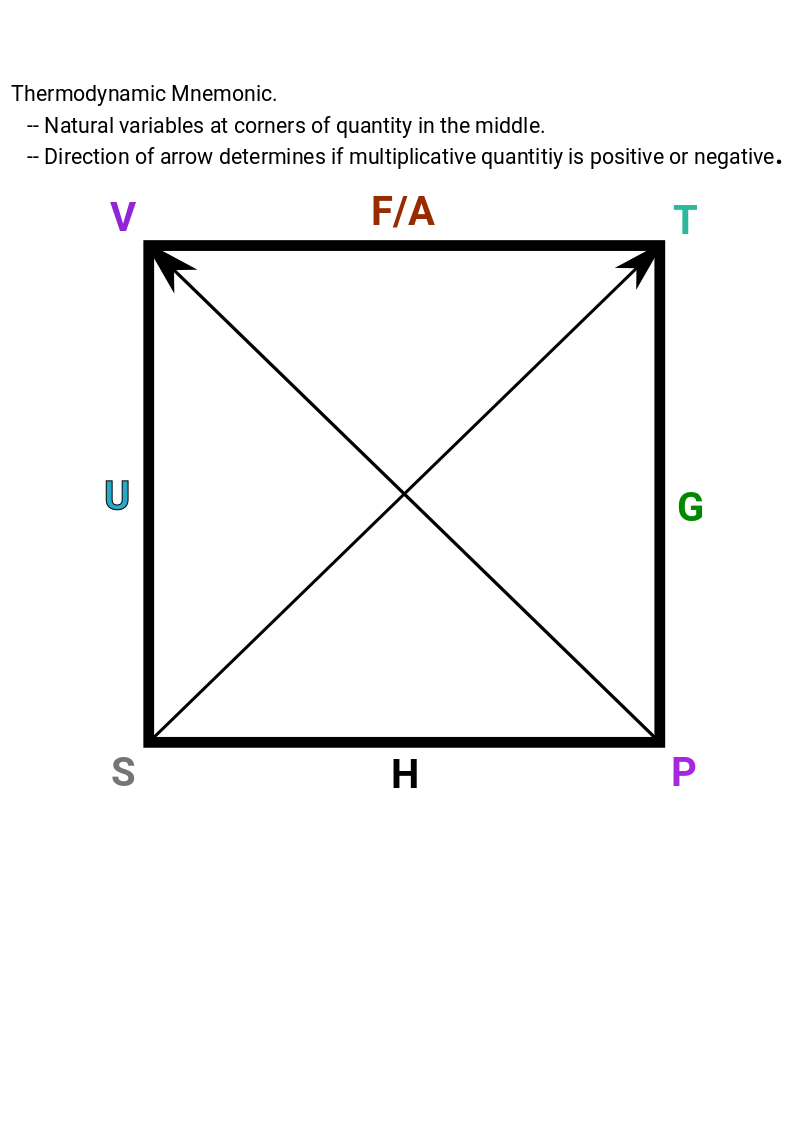
\includegraphics[width=.9\linewidth]{Images/Thermodynamic_mnemonic.png}

\section{Useful Notes}
\label{sec-4}
\subsection{Org-mode}
\label{sec-4-1}
\begin{minted}[]{elisp}
(setq org-latex-create-formula-image-program 'dvipng)
\end{minted}

\subsection{Physics}
\label{sec-4-2}
\subsubsection{Hartree-Fock}
\label{sec-4-2-1}
\begin{itemize}
\item Hartree-Fock is a method of calculating the energy of a configuration
with exact exchange.
\item This is done by essentially putting everything we don't know into the
kinetic energy functional.
\item Hamiltonian is split into contributions:
\begin{itemize}
\item \[\hat{H} = \hat{T} + \hat{V}_{ \text{ext} } + \hat{G}\]
\item $\hat{G} = \hat{J} - \hat{K}$
\item $\hat{J}$ is the coulombic interaction:
\item \[ \bra{ \mathbf{r} } \hat{J} \ket{ \mathbf{n} } = \int \frac{ \bra{\mathbf{r}}\ket{n} }{|\mathbf{r} - \mathbf{r'}  |}d\mathbf{r} \]
\item So \[ E_{\text{H}} = \int \frac{\rho{\mathbf{r}\rho{\mathbf{r}'}}}{|\mathbf{r} - \mathbf{r'}|}\]
\item This includes fictitious self-interaction of electron density.
\item The Exchange functional removes this part, thus lowering the energy
\end{itemize}

\item This method is used in Hybrid DFT. This corrects band gaps mainly. But
there are also problems.
\end{itemize}

\section{org-mode cheat sheet}
\label{sec-5}
\begin{itemize}
\item New TODO: M-<shift>-<ret>
\item Done TODO: C-c C-t
\item Links: [[][]] [link] then [description]
\item Open link: Move over cursor and do C-c C-o
\item Link to local files:
\begin{itemize}
\item Open file (C-x C-f) then do C-c l,
\item then go back to org file and do C-c C-l (e.g. \href{file:///home/tigany/Documents/docs/PhDPaperSummary/upgrade_rep_plus_notes.tex}{Upgrade$_{\text{report}}$$_{\text{plus}}$$_{\text{notes}}$})
\end{itemize}
\item To remove window in buffer C-x 0
\item Overview of document <shift>-<TAB> to condense to titles.
\item Can have global todo list
\item <s TAB expands to a ‘src’ code block.
\item <l TAB expands to a 'latex' code block. '
\end{itemize}


\begin{itemize}
\item If I want more help I can go to the \href{https://orgmode.org/manual/}{org-mode manual}
\end{itemize}


\section{Bibliography}
\label{sec-6}
\label{bibliography-link}

\bibliographystyle{plain}
\bibliography{bibliography/org-refs}
% Emacs 25.3.1 (Org mode 8.2.10)
\end{document}
